%\VignetteIndexEntry{Data and analysis in picante}
%\VignettePackage{picante}
\documentclass[12pt]{article}
\usepackage{amssymb,amsmath}
\usepackage{geometry}
\geometry{letterpaper}
\usepackage{graphicx}
\usepackage{url}

\title{An introduction to the picante package}
\author{Steven Kembel (steve.kembel@gmail.com)}
\date{April 2010}

\usepackage{Sweave}
\begin{document}


\maketitle

\tableofcontents

\section{Installing picante}

The picante homepage is located at \url{http://picante.r-forge.r-project.org}. From within R, you can install the latest version of picante by typing "\texttt{install.packages(picante, dependencies=TRUE)}". Typing "\texttt{help(functionName)}" will display documentation for any function in the package.

Once the package has been installed, it can be loaded by typing:

\begin{Schunk}
\begin{Sinput}
> library(picante)
\end{Sinput}
\end{Schunk}

\section{Data formats in picante}

Most analyses in picante work with one of three types of data. The picante package includes a dataset that contains examples of each of these data types. Loading the dataset creates an object named phylocom that include some artificial data included with the Phylocom (Webb et al. 2008) software. We'll create new objects containing each data type so we don't have to type the full name every time:

\begin{Schunk}
\begin{Sinput}
> data(phylocom)
> names(phylocom)
\end{Sinput}
\begin{Soutput}
[1] "phylo"  "sample" "traits"
\end{Soutput}
\begin{Sinput}
> phy <- phylocom$phylo
> comm <- phylocom$sample
> traits <- phylocom$traits
\end{Sinput}
\end{Schunk}

\subsection{Phylogenies}

Picante uses the \texttt{phylo} format implemented in the \texttt{ape} package to represent phylogenetic relationships among taxa. The format itself is documented at the \texttt{ape} homepage (\url{http://ape.mpl.ird.fr/}). If you have a phylogeny in Newick or Nexus format it can be imported into R with the \texttt{read.tree} or \texttt{read.nexus} functions.

\begin{Schunk}
\begin{Sinput}
> phy
\end{Sinput}
\begin{Soutput}
Phylogenetic tree with 32 tips and 31 internal nodes.

Tip labels:
  sp1, sp2, sp3, sp4, sp5, sp6, ...
Node labels:
  A, B, C, D, E, F, ...

Rooted; includes branch lengths.
\end{Soutput}
\end{Schunk}

\subsection{Community data}

Picante uses the same community data format as the \texttt{vegan} package - a matrix or data.frame with sites/samples in the rows and taxa in the columns. The elements of this data frame should be numeric values indicating the abundance or presence/absence (0/1) of taxa in different samples.

One important thing to note is that most functions in picante will use the labels on columns in the community data set to match community and phylogenetic data together. You need to make sure your column names are present and match the tip labels of the phylogeny or your analysis may not work. Most functions in picante do basic error checking and will report when there are mismatches between the data present in the community and phylogenetic data sets. Similarly, your communities/sites/samples can be given informative names, and these should be contained in the row labels, not in a column of the data.frame.

\begin{Schunk}
\begin{Sinput}
> comm
\end{Sinput}
\begin{Soutput}
        sp1 sp10 sp11 sp12 sp13 sp14 sp15 sp17 sp18 sp19 sp2 sp20 sp21
clump1    1    0    0    0    0    0    0    0    0    0   1    0    0
clump2a   1    2    2    2    0    0    0    0    0    0   1    0    0
clump2b   1    0    0    0    0    0    0    2    2    2   1    2    0
clump4    1    1    0    0    0    0    0    2    2    0   1    0    0
even      1    0    0    0    1    0    0    1    0    0   0    0    1
random    0    0    0    1    0    4    2    3    0    0   1    0    0
        sp22 sp24 sp25 sp26 sp29 sp3 sp4 sp5 sp6 sp7 sp8 sp9
clump1     0    0    0    0    0   1   1   1   1   1   1   0
clump2a    0    0    0    0    0   1   1   0   0   0   0   2
clump2b    0    0    0    0    0   1   1   0   0   0   0   0
clump4     0    0    2    2    0   0   0   0   0   0   0   1
even       0    0    1    0    1   0   0   1   0   0   0   1
random     1    2    0    0    0   0   0   2   0   0   0   0
\end{Soutput}
\begin{Sinput}
> class(comm)
\end{Sinput}
\begin{Soutput}
[1] "matrix" "array" 
\end{Soutput}
\begin{Sinput}
> colnames(comm)
\end{Sinput}
\begin{Soutput}
 [1] "sp1"  "sp10" "sp11" "sp12" "sp13" "sp14" "sp15" "sp17" "sp18"
[10] "sp19" "sp2"  "sp20" "sp21" "sp22" "sp24" "sp25" "sp26" "sp29"
[19] "sp3"  "sp4"  "sp5"  "sp6"  "sp7"  "sp8"  "sp9" 
\end{Soutput}
\begin{Sinput}
> rownames(comm)
\end{Sinput}
\begin{Soutput}
[1] "clump1"  "clump2a" "clump2b" "clump4"  "even"    "random" 
\end{Soutput}
\end{Schunk}

\subsection{Trait data}

Trait data include any kind of data associated with the taxa present in a phylogeny. Most functions in picante work with trait data represented as a vector (for individual traits) or data.frame. The documentation for individual functions will explain which data format is expected.

When trait data are contained in a data.frame, taxa are in rows and different traits are in columns. As with community data, rows must be labelled and the labels must match taxa names in the phylogeny. If your trait data.frame does not have row labels, it is assumed that the rows are sorted in the same order as the tip labels of the phylogeny.

When trait data are contained in a vector, the vector must be labelled, or it will be assumed that the elements of the vector are in the same order as the tip labels of the phylogeny. There is a utility function in picante that will turn columns of a data frame into vectors maintaining taxa labels that you can use if you have a data.frame and need a vector for a particular analysis:


\section{Visualizing trees and data}

One of the main advantages of using R is that a suite of graphical and statistical tools are included. Now that we've loaded our data sets, we can use some of those tools to visualize them. Remember that we have three objects containing the community (\texttt{comm}), phylogeny (\texttt{phy}), and trait (\texttt{traits}) data sets.

Most functions in \texttt{picante} assume that the community, trait and phylogeny data sets contain the same taxa arranged in the same order. Functions that are affected by this assumption will attempt to automatically match the taxa labels in different data sets, and will report taxa that are not present in both data sets.

Let's see how taxa from the six communities in the Phylocom example data set are arranged on the tree. To do this, we first need to prune the phylogeny to include only the species that actually occurred in some community.

\begin{Schunk}
\begin{Sinput}
> prunedphy <- prune.sample(comm, phy)
> prunedphy
\end{Sinput}
\begin{Soutput}
Phylogenetic tree with 25 tips and 24 internal nodes.

Tip labels:
  sp1, sp2, sp3, sp4, sp5, sp6, ...
Node labels:
  A, B, C, D, E, F, ...

Rooted; includes branch lengths.
\end{Soutput}
\end{Schunk}

The following commands set up the layout of the plot to have 2 rows and 3 columns, and then plot a black dot for the species present in each of the six communities:

\begin{Schunk}
\begin{Sinput}
> par(mfrow = c(2, 3))
> for (i in row.names(comm)) {
+ plot(prunedphy, show.tip.label = FALSE, main = i)
+ tiplabels(tip = which(prunedphy$tip.label %in% names(which(comm [i, ] > 0))),
+           pch=19, cex=2)
+ }
\end{Sinput}
\end{Schunk}
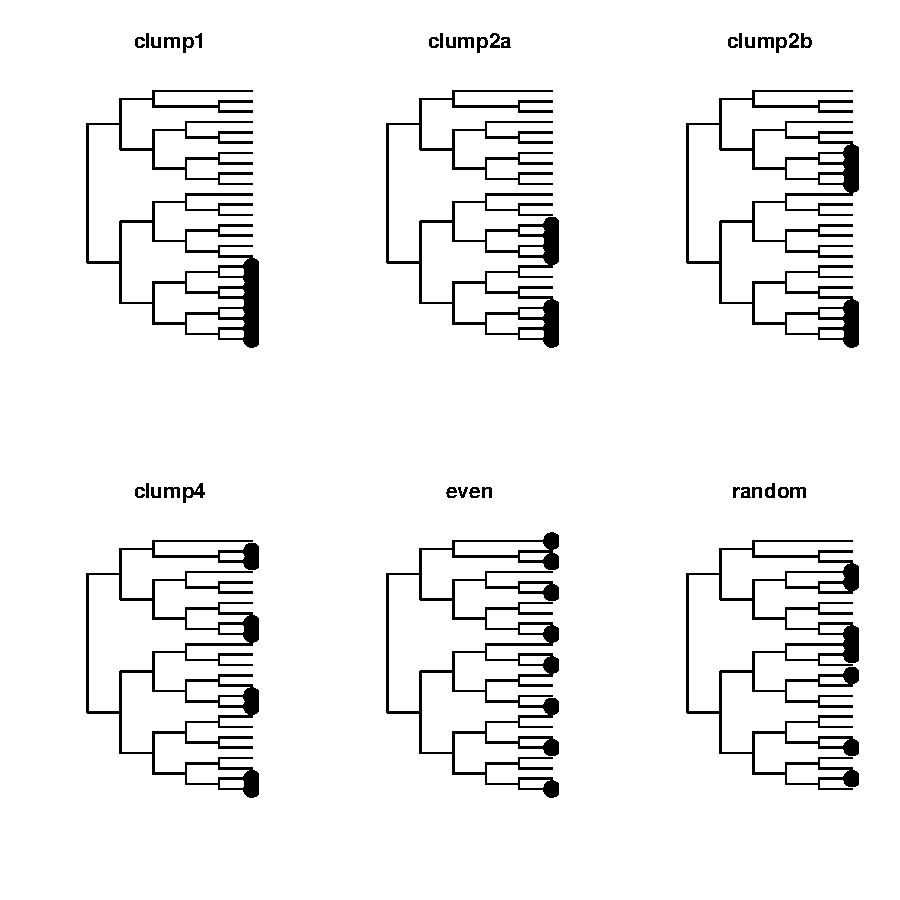
\includegraphics{picante-intro-007}

Similarly, let's visualize the trait values on the trees by plotting a different color for each trait value. The arguments to the \texttt{tiplabels} function give each trait value a unique color and adjust the size of the trait symbols.

\begin{Schunk}
\begin{Sinput}
> par(mfrow=c(2,2))
> for (i in names(traits)) {
+ 	plot(phy, show.tip.label=FALSE, main=i)
+ 	tiplabels(pch=22, col=traits[,i]+1, bg=traits[,i]+1, cex=1.5)
+ }
\end{Sinput}
\end{Schunk}
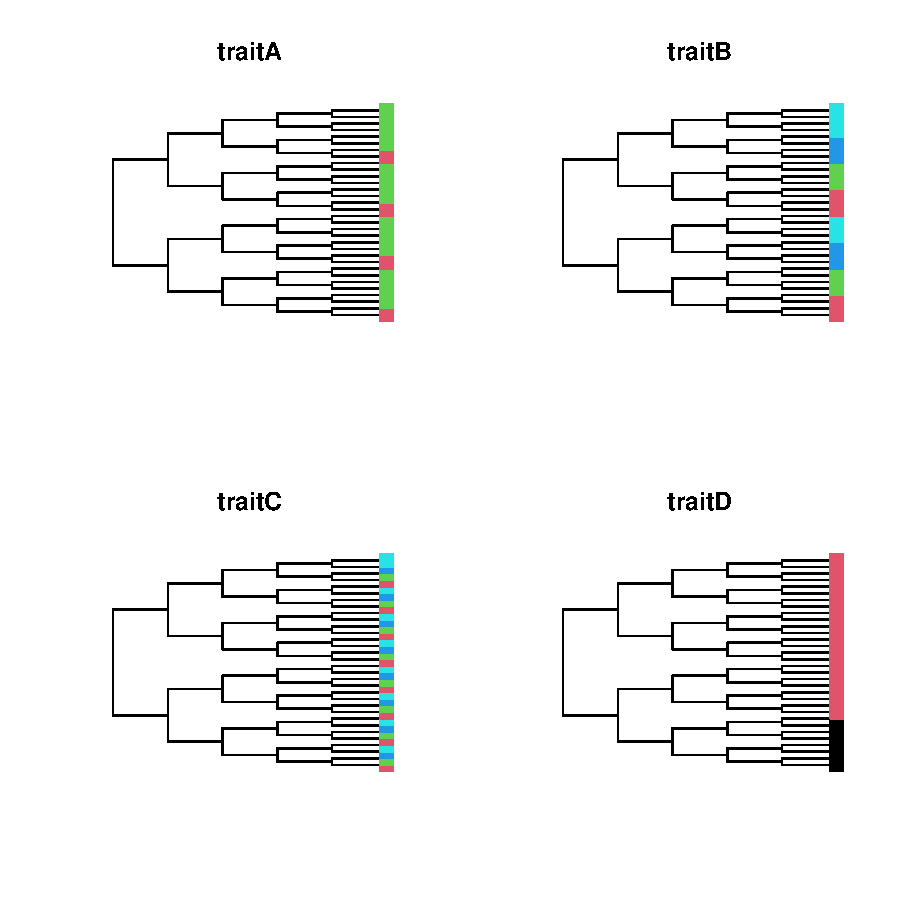
\includegraphics{picante-intro-008}

Looking at these plots, which communities would you expect to be phylogenetically clustered or phylogenetically even? Which of the four traits do you think has the greatest amount of phylogenetic signal?

\section{Community phylogenetic structure}

\subsection{Phylogenetic diversity}

One of the earliest measures of phylogenetic relatedness in ecological communities was the phylogenetic diversity (PD) index proposed by Faith (1992). Faith's PD is defined as the total branch length spanned by the tree including all species in a local community. The \texttt{pd} function returns two values for each community, the PD and the species richness (SR).

\begin{Schunk}
\begin{Sinput}
> pd.result <- pd(comm, phy, include.root=TRUE)
> pd.result
\end{Sinput}
\begin{Soutput}
        PD SR
clump1  16  8
clump2a 17  8
clump2b 18  8
clump4  22  8
even    30  8
random  27  8
\end{Soutput}
\end{Schunk}

Looking at these results, we can see that the communities where taxa are clumped on the phylogeny tend to have a lower PD, because the species in these communities capture only a small part of the total phylogenetic diversity present in the phylogeny.

\subsection{MPD, MNTD,  $SES_{MPD}$ and $SES_{MNTD}$}

Another way of thinking about the phylogenetic relatedness of species in a community is to ask 'how closely related are the average pair of species or individuals in a community?', and relate the patterns we observe to what we'd expect under various null models of evolution and community assembly. These types of questions are addressed by the measures of community phylogenetic structure such as MPD, MNTD, NRI and NTI described by Webb et al. (2002) and implemented in Phylocom (Webb et al. 2008).

The function \texttt{mpd} will calculate the mean pairwise distance (MPD) between all species in each community. Similarly, the \texttt{mntd} function calculates the mean nearest taxon distance (MNTD), the mean distance separating each species in the community from its closest relative. The \texttt{mpd} and \texttt{mntd} functions differs slightly from the \texttt{pd} function in that they take a distance matrix as input rather than a phylogeny object. A \texttt{phylo} object can be converted to a interspecific phylogenetic distance matrix using the \texttt{cophenetic} function. Since the \texttt{mpd} and \texttt{mntd} functions can use any distance matrix as input, we could easily calculate trait diversity measures by substituting a trait distance matrix for the phylogenetic distance matrix.

Measures of `standardized effect size' of phylogenetic community structure can be calculated for MPD and MNTD by compared observed phylogenetic relatedness to the pattern expected under some null model of phylogeny or community randomization. Standardized effect sizes describe the difference between phylogenetic distances in the observed communities versus null communities generated with some randomization method, divided by the standard deviation of phylogenetic distances in the null data:

\[SES_{metric} =  \frac{ Metric_{observed} - mean(Metric_{null}) }{sd(Metric_{null})}\]

\noindent Phylocom users will be familiar with the measures NRI and NTI; $SES_{MPD}$ and $SES_{MNTD}$ are equivalent to -1 times NRI and NTI, respectively, when these functions are run with a phylogenetic distance matrix.

Several different null models can be used to generate the null communities that we compare observed patterns to. These include randomizations of the tip labels of the phylogeny, and various community randomizations that can hold community species richness and/or species occurrence frequency constant. These are described in more detail in the help files, as well as in the Phylocom manual. Let's calculate some of these measures of community phylogenetic structure for our example data set. We will use a simple null model of randomly shuffling tip labels across the tips of the phylogeny. For a 'real' analysis we'd want to use a much higher number of runs:

\begin{Schunk}
\begin{Sinput}
> phydist <- cophenetic(phy)
> ses.mpd.result <- ses.mpd(comm, phydist, null.model="taxa.labels",
+                           abundance.weighted=FALSE, runs=99)
> ses.mpd.result
\end{Sinput}
\begin{Soutput}
        ntaxa  mpd.obs mpd.rand.mean mpd.rand.sd mpd.obs.rank
clump1      8 4.857143      8.312410   0.3033181          1.0
clump2a     8 6.000000      8.323954   0.3088843          1.0
clump2b     8 7.142857      8.344877   0.2927416          1.0
clump4      8 8.285714      8.387446   0.3251071         30.0
even        8 8.857143      8.282828   0.4138531         99.5
random      8 8.428571      8.333333   0.3159972         54.5
          mpd.obs.z mpd.obs.p runs
clump1  -11.3915627     0.010   99
clump2a  -7.5237025     0.010   99
clump2b  -4.1060787     0.010   99
clump4   -0.3129172     0.300   99
even      1.3877257     0.995   99
random    0.3013891     0.545   99
\end{Soutput}
\begin{Sinput}
> ses.mntd.result <- ses.mntd(comm, phydist, null.model="taxa.labels",
+                             abundance.weighted=FALSE, runs=99)
> ses.mntd.result
\end{Sinput}
\begin{Soutput}
        ntaxa mntd.obs mntd.rand.mean mntd.rand.sd mntd.obs.rank
clump1      8        2       4.676768    0.6198796           1.0
clump2a     8        2       4.719697    0.5454739           1.0
clump2b     8        2       4.780303    0.6460957           1.0
clump4      8        2       4.681818    0.6446584           1.0
even        8        6       4.661616    0.7216700          99.0
random      8        5       4.797980    0.6687988          58.5
        mntd.obs.z mntd.obs.p runs
clump1  -4.3182061      0.010   99
clump2a -4.9859345      0.010   99
clump2b -4.3032369      0.010   99
clump4  -4.1600611      0.010   99
even     1.8545649      0.990   99
random   0.3020643      0.585   99
\end{Soutput}
\end{Schunk}

\noindent The output includes the following columns:

\begin{itemize}
\item{ \texttt{ntaxa}}	 Number of taxa in community
\item{ \texttt{mpd.obs}}	 Observed mpd in community
\item{ \texttt{mpd.rand.mean}}	 Mean mpd in null communities
\item{ \texttt{mpd.rand.sd}}	 Standard deviation of mpd in null communities
\item{ \texttt{mpd.obs.rank}}	 Rank of observed mpd vs. null communities
\item{ \texttt{mpd.obs.z}}	 Standardized effect size of mpd vs. null communities (equivalent to -NRI)
\item{ \texttt{mpd.obs.p}}	 P-value (quantile) of observed mpd vs. null communities (= mpd.obs.rank / runs + 1)
\item{ \texttt{runs}}	 Number of randomizations
\end{itemize}

Positive $SES$ values (\texttt{mpd.obs.z} > 0) and high quantiles (\texttt{mpd.obs.p} > 0.95) indicate phylogenetic evenness, or a greater phylogenetic distance among co-occurring species than expected. Negative SES values and low quantiles (\texttt{mpd.obs.p} < 0.05) indicate phylogenetic clustering, or small phylogenetic distances among co-occurring species than expected. MPD is generally thought to be more sensitive to tree-wide patterns of phylogenetic clustering and eveness, while MNTD is more sensitive to patterns of evenness and clustering closer to the tips of the phylogeny. For example, community 'clump4' contains species that are spread randomly across the entire tree ($SES_{MPD}$ close to zero) but phylogenetically clustered towards the tips (negative $SES_{MNTD}$ and \texttt{mntd.obs.p} in the low quantiles of the null distribution).

All of these measures can incorporate abundance information when available using the \texttt{abundance.weighted} argument. This will change the interpretation of these metrics from the mean phylogenetic distances among species, to the mean phylogenetic distances among individuals.

\subsection{Phylogenetic beta diversity}

We can measure patterns of phylogenetic relatedness among communities in a manner similar to the within-community measures described above. The \texttt{comdist} and \texttt{comdistnt} functions measure the among-community equivalent of MPD and MNTD, the mean phylogenetic distance or mean nearest taxon distance between pairs of species drawn from two distinct communities.

Phylogenetic beta diversity measures can be used with any method based on measuring among-community distances. For example, they could be used in a cluster analysis or phyloordination to group communities based on their evolutionary similarity, or they could be compared with spatial or environmental distances separating communities using a Mantel test. The code below calculates MPD between pairs of communities, and uses these phylogenetic distances to cluster communities based on their phylogenetic similarity:

\begin{Schunk}
\begin{Sinput}
> comdist.result <- comdist(comm, phydist)
\end{Sinput}
\begin{Soutput}
[1] "Dropping taxa from the distance matrix because\n     they are not present in the community data:"
[1] "sp16" "sp23" "sp27" "sp28" "sp30" "sp31" "sp32"
\end{Soutput}
\begin{Sinput}
> comdist.result
\end{Sinput}
\begin{Soutput}
         clump1 clump2a clump2b  clump4    even
clump2a 6.12500                                
clump2b 7.12500 7.62500                        
clump4  8.06250 7.62500 7.62500                
even    8.06250 8.06250 8.06250 7.87500        
random  7.81250 7.68750 7.93750 8.12500 8.03125
\end{Soutput}
\begin{Sinput}
> comdist.clusters <- hclust(comdist.result)
> plot(comdist.clusters)
\end{Sinput}
\end{Schunk}
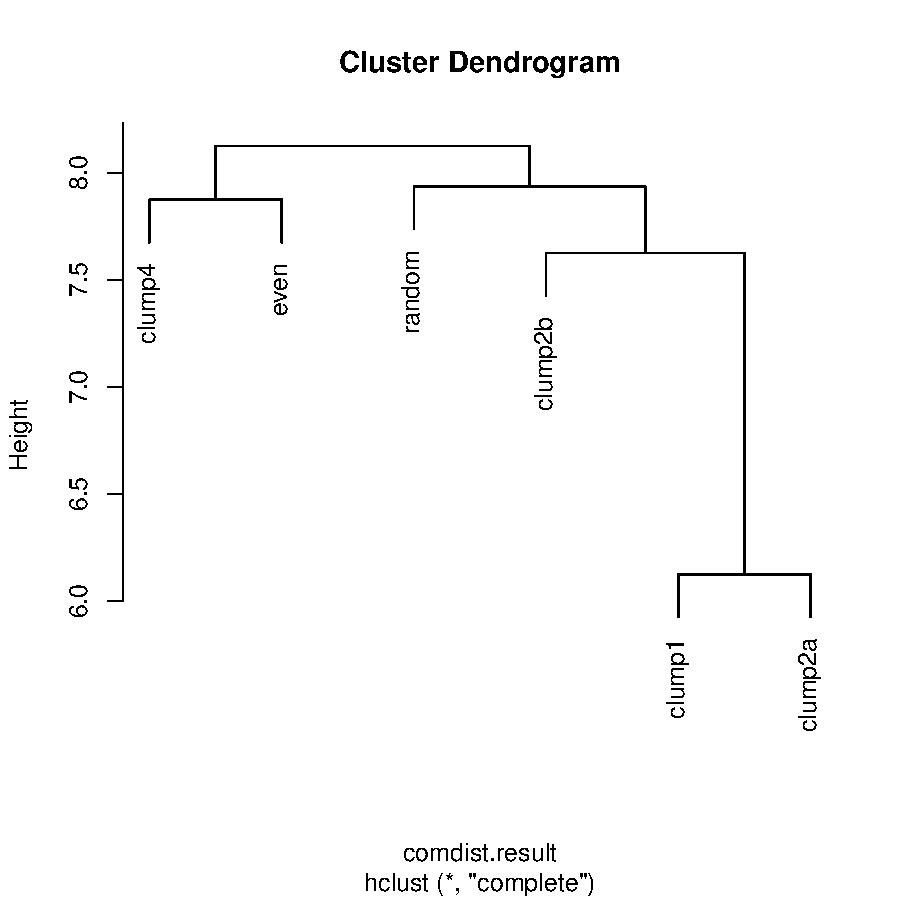
\includegraphics{picante-intro-012}

\section{Comparative analyses}

\subsection{Phylogenetic signal}

The idea of phylogenetic niche conservatism (the ecological similarity of closely related species) has attracted a lot of attention recently, for example in the widely used framework of inferring community assembly processes based on knowledge of community phylogenetic structure plus the phylogenetic conservatism of traits. (Webb et al. 2002).

Phylogenetic signal is a quantitative measure of the degree to which phylogeny predicts the ecological similarity of species. The $K$ statistic is a measure of phylogenetic signal that compares the observed signal in a trait to the signal under a Brownian motion model of trait evolution on a phylogeny (Blomberg et al. 2003). $K$ values of 1 correspond to a Brownian motion process, which implies some degree of phylogenetic signal or conservatism. $K$ values closer to zero correspond to a random or convergent pattern of evolution, while $K$ values greater than 1 indicate strong phylogenetic signal and conservatism of traits. The statistical significance of phylogenetic signal can be evaluated by comparing observed patterns of the variance of independent contrasts of the trait to a null model of shuffling taxa labels across the tips of the phylogeny.

These tests are implemented in the \texttt{Kcalc}, \texttt{phylosignal}, and \texttt{multiPhylosignal} functions. All of these functions assume the trait data are in the same order as the phylogeny tip.labels. Let's make sure the Phylocom trait data are in this order and then measure phylogenetic signal in these data.

\begin{Schunk}
\begin{Sinput}
> traits <- traits[phy$tip.label,]
> multiPhylosignal(traits,phy)
\end{Sinput}
\begin{Soutput}
               K PIC.variance.obs PIC.variance.rnd.mean PIC.variance.P
traitA 0.8905609       0.05396825             0.1249901          0.003
traitB 2.9340184       0.10920635             0.8344980          0.001
traitC 0.5149502       0.62222222             0.8362014          0.063
traitD 4.3536696       0.01103943             0.1253782          0.001
       PIC.variance.Z
traitA      -3.571045
traitB      -5.288878
traitC      -1.600700
traitD      -5.817005
\end{Soutput}
\end{Schunk}

The higher the $K$ statistic, the more phylogenetic signal in a trait. \texttt{PIC.variance.P} is the quantile of the observed phylogenetically independent contrast variance versus the null distribution, which can be used as a 1-tailed P-value to test for greater phylogenetic signal than expected. Traits with \texttt{PIC.variance.P} < 0.05 have non-random phylogenetic signal.

\section{Literature cited}

\begin{itemize}
\item{Blomberg, S. P., T. Garland, Jr., and A. R. Ives. 2003. Testing for phylogenetic signal in comparative data: behavioral traits are more labile. Evolution 57:717-745.}
\item{Faith, D.P. 1992. Conservation evaluation and phylogenetic diversity. Biological Conservation, 61:1-10.}
\item{Webb, C., D. Ackerly, M. McPeek, and M. Donoghue. 2002. Phylogenies and community ecology. Annual Review of Ecology and Systematics 33:475-505.}
\item{Webb, C.O., Ackerly, D.D., and Kembel, S.W. 2008. Phylocom: software for the analysis of phylogenetic community structure and trait evolution. Bioinformatics 18:2098-2100. }
\end{itemize}

\end{document}
